% !TeX program = xelatex
% Paper-first report; original sonnyhcl/beamerthemefdu in vendor-fdu/ (Apache-2.0).
\documentclass[aspectratio=169,12pt,fontset=none]{ctexbeamer}
\usepackage{lmodern,fontspec,amsmath,amssymb,booktabs,array,tabularx,graphicx,tikz}
\setsansfont{Arial}\setmainfont{Arial}
\setCJKmainfont{Microsoft YaHei}[BoldFont=Microsoft YaHei Bold]
\setCJKsansfont{Microsoft YaHei}[BoldFont=Microsoft YaHei Bold]
\setCJKmonofont{Microsoft YaHei}
\usetikzlibrary{arrows.meta,positioning,calc,backgrounds,fit}
\makeatletter\def\input@path{{vendor-fdu/}}\makeatother
\usetheme{fdu}
\usefonttheme{professionalfonts}
% Preserve native FDU layouts; configure watermark opacity and author metadata.
% The upstream .sty remains byte-for-byte unchanged.
\makeatletter
\expandafter\patchcmd\csname beamer@@tmpl@background canvas\endcsname{opacity=.05}{opacity=.022}{}{\PackageError{course}{Cannot configure FDU watermark}{}}
\expandafter\patchcmd\csname beamer@@tmpl@footline\endcsname{\insertshortauthor~(\insertshortinstitute)}{\insertshortauthor}{}{\PackageError{course}{Cannot configure author footer}{}}
\makeatother
\graphicspath{{resources/}{../../data/results/dominance_figures/}{../../data/results/kreach_figures/}}
\definecolor{Navy}{HTML}{132A46}
\definecolor{FBlue}{HTML}{1766A3}
\definecolor{Teal}{HTML}{008B80}
\definecolor{Gold}{HTML}{C49A3B}
\definecolor{Muted}{HTML}{62758B}
\definecolor{Line}{HTML}{D8E2EB}
\definecolor{Edge}{HTML}{91A4B6}
\definecolor{Light}{HTML}{F1F5F8}
\definecolor{Alert}{HTML}{AE4D4D}
\setbeamercolor{normal text}{fg=Navy,bg=white}
\setbeamercolor{structure}{fg=FBlue}
\setbeamercolor{frametitle}{fg=white,bg=FBlue}
\setbeamercolor{title}{fg=white,bg=FBlue}
\setbeamercolor{palette primary}{fg=white,bg=FBlue}
\setbeamercolor{palette secondary}{fg=white,bg=Navy}
\setbeamercolor{palette tertiary}{fg=white,bg=Navy}
\setbeamercolor{title in head/foot}{fg=white,bg=Navy!95}
\setbeamercolor{block body}{fg=Navy,bg=Light}
\setbeamercolor{alerted text}{fg=Alert}
\setbeamerfont{frametitle}{size=\Large,series=\bfseries}
\setbeamerfont{title}{size=\Large,series=\bfseries}
\setbeamerfont{subtitle}{size=\normalsize}
\setbeamerfont{author}{size=\normalsize}
\setbeamerfont{institute}{size=\footnotesize}
\setbeamerfont{date}{size=\footnotesize}
\setbeamersize{text margin left=8mm,text margin right=8mm}
\setbeamertemplate{navigation symbols}{}
\setlength{\parskip}{.15em}
\newcommand{\Key}[1]{\par\vspace{1mm}\begin{beamercolorbox}[wd=\textwidth,sep=1.8mm,rounded=true]{block body}\fontsize{11}{13}\selectfont #1\end{beamercolorbox}}
\newcommand{\T}[1]{{\color{Teal}\bfseries #1}}
\newcommand{\G}[1]{{\color{Gold}\bfseries #1}}
\newcommand{\Micro}[1]{{\fontsize{11}{14}\selectfont #1}}
\renewcommand{\arraystretch}{1.22}
\newcommand{\PaperGraph}[2][1]{%
\begin{tikzpicture}[x=10mm,y=8mm,vertex/.style={circle,draw=Line,fill=white,minimum size=6.5mm,inner sep=0pt,font=\normalsize},core/.style={vertex,draw=Gold,fill=Gold!12,line width=1.1pt},every edge/.style={-{Stealth[length=1.8mm]},draw=Edge,line width=.7pt}]
\ifnum#1=0\tikzset{core/.style={vertex}}\fi
\node[vertex] (a) at (0,0) {a};
\node[core] (b) at (1.2,0) {b};
\node[vertex] (c) at (1.8,1.15) {c};
\node[core] (d) at (2.4,0) {d};
\node[vertex] (e) at (3.6,0) {e};
\node[vertex] (f) at (3.6,-1.15) {f};
\node[core] (g) at (4.8,0) {g};
\node[vertex] (h) at (5.4,1.15) {h};
\node[core] (i) at (6,0) {i};
\node[vertex] (j) at (7.2,0) {j};
\begin{scope}[on background layer]
\draw[every edge] (a) -- (b);
\draw[every edge] (c) -- (b);
\draw[every edge] (b) -- (d);
\draw[every edge] (d) -- (c);
\draw[every edge] (d) -- (e);
\draw[every edge] (e) -- (g);
\draw[every edge] (d) -- (f);
\draw[every edge] (g) -- (f);
\draw[every edge] (g) -- (h);
\draw[every edge] (g) -- (i);
\draw[every edge] (i) -- (j);
\foreach \u/\v in {#2}{\draw[-{Stealth[length=2.1mm]},draw=FBlue,line width=1.7pt] (\u) -- (\v);}
\end{scope}
\end{tikzpicture}}
\newcommand{\DominanceGraph}[2][1]{%
\begin{tikzpicture}[x=10mm,y=8mm,vertex/.style={circle,draw=Line,fill=white,minimum size=6.5mm,inner sep=0pt,font=\normalsize},core/.style={vertex,draw=Gold,fill=Gold!12,line width=1.1pt},every edge/.style={-{Stealth[length=1.8mm]},draw=Edge,line width=.7pt}]
\ifnum#1=0\tikzset{core/.style={vertex}}\fi
\node[vertex] (a) at (0,0) {a};
\node[core] (b) at (1.2,0) {b};
\node[vertex] (c) at (1.8,1.15) {c};
\node[core] (d) at (2.4,0) {d};
\node[vertex] (e) at (3.6,0) {e};
\node[vertex] (f) at (3.6,-1.15) {f};
\node[core] (g) at (4.8,0) {g};
\node[vertex] (h) at (5.4,1.15) {h};
\node[core] (i) at (6,0) {i};
\node[vertex] (j) at (7.2,0) {j};
\begin{scope}[on background layer]
\draw[every edge] (a) -- (b);
\draw[every edge] (c) -- (b);
\draw[every edge] (b) -- (d);
\draw[every edge] (d) -- (c);
\draw[every edge] (d) -- (e);
\draw[every edge] (e) -- (g);
\draw[every edge] (d) -- (f);
\draw[every edge] (g) -- (f);
\draw[every edge] (g) -- (h);
\draw[every edge] (g) -- (i);
\draw[every edge] (i) -- (j);
\draw[-{Stealth[length=2mm]},draw=Teal,line width=1.3pt] (c) to[bend left=25] (d);
\foreach \u/\v in {#2}{\draw[-{Stealth[length=2.1mm]},draw=FBlue,line width=1.7pt] (\u) -- (\v);}
\end{scope}
\end{tikzpicture}}
\newcommand{\WikiPruningSpeed}{1.28}
\newcommand{\WikiJoinSpeed}{1.13}

\title[K-hop 可达性查询]{K-hop 可达性查询}
\subtitle{K-Reach 论文分析与阈值支配剪枝}
\author[第十三组]{第十三组}
\institute[]{《图数据管理与挖掘》课程期中汇报}
\date[]{}
\hypersetup{pdftitle={K-hop 可达性查询：K-Reach 论文分析与阈值支配剪枝},pdfauthor={第十三组},pdfsubject={K-hop 可达性查询论文精读与改进验证},colorlinks=true,urlcolor=FBlue,linkcolor=white}
\begin{document}
\begin{frame}
\titlepage
\end{frame}
\section{背景与问题}
\begin{frame}{研究背景与问题定义}
社交关系分析、信任关系检索等任务，常需要限制关系链的长度。对大量重复查询，逐次运行 BFS 会反复访问相同的局部结构。
\par\vspace{2mm}
\begin{columns}[c,onlytextwidth]
\column{.45\textwidth}
\begin{block}{K-hop 可达性查询}
给定有向无权图 $G=(V,E)$、节点 $s,t$ 和跳数上限 $k$，判断是否存在至多 $k$ 条边的路径：
\[
Q(s,t,k)=[d_G(s,t)\le k].
\]
\end{block}
\column{.51\textwidth}\centering
\resizebox{\linewidth}{!}{\PaperGraph[0]{a/b,b/d,d/e,e/g}}\par\vspace{2mm}
$d(a,g)=4$\par
$k=3$：不可达 \qquad $k=4$：可达
\end{columns}
\end{frame}

\section{论文方法}
\begin{frame}{K-Reach 的研究思路与框架}
\noindent
{\fontsize{10.5}{13}\selectfont
\textbf{K-Reach: Who is in Your Small World}\par
James Cheng, Zechao Shang, Hong Cheng, Haixun Wang, Jeffrey Xu Yu\par
\emph{PVLDB} 5(11):1292–1303, 2012.}\par\vspace{3mm}
论文通过顶点覆盖，将任意端点的跳数查询转化为核心节点之间的距离判定。
\par\vspace{2mm}
\begin{columns}[c,onlytextwidth]
\column{.30\textwidth}
\begin{block}{顶点覆盖}
选择核心集合，使覆盖外端点一跳接入核心。
\end{block}
\column{.03\textwidth}\centering$\rightarrow$
\column{.30\textwidth}
\begin{block}{三档距离索引}
保存 $k-2$、$k-1$、$k$ 三个阈值需要的信息。
\end{block}
\column{.03\textwidth}\centering$\rightarrow$
\column{.30\textwidth}
\begin{block}{四类查询}
根据起点和终点是否在核心中，选择查询方式。
\end{block}
\end{columns}
\par\vspace{2mm}
这种设计兼顾了索引规模与查询效率，避免保存所有完整距离。
\end{frame}

\begin{frame}{关键技术一：用顶点覆盖连接查询端点}
\begin{columns}[c,onlytextwidth]
\column{.60\textwidth}\centering
\resizebox{\linewidth}{!}{\PaperGraph{b/d,g/i}}\par\vspace{2mm}
覆盖集合 $S=\{b,d,g,i\}$
\column{.36\textwidth}
顶点覆盖要求每条边至少一端在 $S$。\par\vspace{2mm}
因此，覆盖外节点之间没有边：
\[
s\notin S\Rightarrow N^+(s)\subseteq S,
\]
\[
t\notin S\Rightarrow N^-(t)\subseteq S.
\]
\end{columns}
\par\vspace{2mm}
论文采用极大匹配的全部端点构造 2-近似顶点覆盖。查询两端各用至多一跳，即可连接到核心。
\end{frame}

\begin{frame}{关键技术二：三档距离索引}
\begin{columns}[c,onlytextwidth]
\column{.37\textwidth}\centering
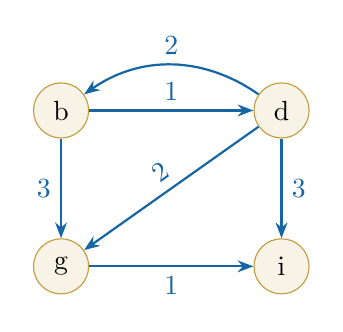
\begin{tikzpicture}[x=14mm,y=12mm,v/.style={circle,draw=Gold,fill=Gold!12,minimum size=7mm},a/.style={-{Stealth[length=2mm]},FBlue,thick}]
\node[v](b)at(0,0){b};\node[v](d)at(2,0){d};
\node[v](g)at(0,-1.65){g};\node[v](i)at(2,-1.65){i};
\draw[a](b)--node[above]{1}(d);
\draw[a](d)to[bend right=35]node[above]{2}(b);
\draw[a](b)--node[left]{3}(g);
\draw[a](d)--node[above,sloped]{2}(g);
\draw[a](d)--node[right]{3}(i);
\draw[a](g)--node[below]{1}(i);
\end{tikzpicture}\par
\Micro{$k=3$ 时的核心索引，省略自环。}
\column{.59\textwidth}
{\fontsize{11}{13}\selectfont
\begin{tabular}{@{}lll@{}}\toprule
核心距离 & 保存的权重 & 两位码\\\midrule
$d\le k-2$ & $k-2$ & 01\\
$d=k-1$ & $k-1$ & 10\\
$d=k$ & $k$ & 11\\
$d>k$ / 不可达 & 无索引边 & 00\\\bottomrule
\end{tabular}}\par\vspace{2mm}
从各核心节点在原图运行 $k$ 限制 BFS，预先构建索引。
\end{columns}
\par\vspace{2mm}
\textbf{编码依据：}端点接入核心各占 0 或 1 跳，剩余预算只有 $k$、$k-1$ 和 $k-2$，因此三档信息足以完成判定。
\end{frame}

\begin{frame}{四类查询及其核心距离预算}
\centering
\begin{tabular}{@{}p{35mm}p{67mm}c@{}}\toprule
端点位置 & 查询的核心点对 & 距离预算\\\midrule
两点都在 $S$ & $(s,t)$ & $k$\\
仅 $s\in S$ & $(s,v)$，$v\in N^-(t)$ & $k-1$\\
仅 $t\in S$ & $(u,t)$，$u\in N^+(s)$ & $k-1$\\
两点都不在 $S$ & $(u,v)$，$u\in N^+(s)$、$v\in N^-(t)$ & $k-2$\\\bottomrule
\end{tabular}\par\vspace{4mm}
对相应核心点对进行检查；只要存在一对满足预算，查询即返回 True。
\end{frame}

\begin{frame}{查询示例：判断 $c$ 能否在三跳内到达 $f$}
\begin{columns}[c,onlytextwidth]
\column{.59\textwidth}\centering
\resizebox{\linewidth}{!}{\PaperGraph{c/b,b/d,d/f}}\par\vspace{2mm}
$c\xrightarrow{1}b\xrightarrow{1}d\xrightarrow{1}f$
\column{.37\textwidth}
\begin{enumerate}
\item $c,f\notin S$，属于第四类。
\item 两端各占一跳，核心预算为 $3-2=1$。
\item $d(b,d)=1$，满足预算，返回 True。
\end{enumerate}
\end{columns}
\par\vspace{2mm}
若终点改为 $h$，则需检查核心点对 $(b,g)$。其距离为 3，超过预算 1，因此返回 False。
\par\vspace{2mm}
当端点连接多个覆盖邻居时，算法仍需枚举这些邻居。我们接下来研究其中可以消去的冗余候选。
\end{frame}


\section{改进方法}

\begin{frame}{改进思路：消去冗余的边界候选}
将覆盖外端点与核心相连的邻居集合称为\textbf{查询边界}。如果一个邻居可达的目标已被另一个邻居覆盖，就可以减少一次候选枚举。
\par\vspace{2mm}
\begin{columns}[c,onlytextwidth]
\column{.54\textwidth}\centering
\resizebox{\linewidth}{!}{
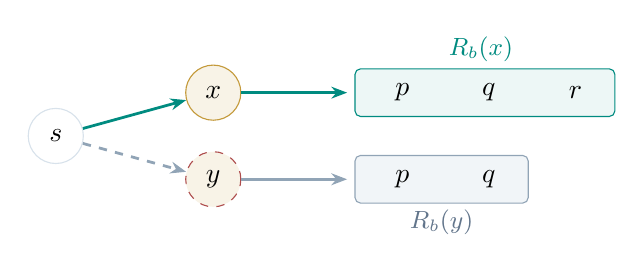
\begin{tikzpicture}[x=10mm,y=5.5mm,
v/.style={circle,draw=Gold,fill=Gold!12,minimum size=7mm,inner sep=0pt,font=\normalsize},
a/.style={-{Stealth[length=2mm]},line width=1pt}]
\node[circle,draw=Line,fill=white,minimum size=7mm](s)at(0,0){$s$};
\node[v](x)at(2,1){$x$};\node[v,draw=Alert,dashed](y)at(2,-1){$y$};
\draw[a,Teal](s)--(x);\draw[a,Edge,dashed](s)--(y);
\filldraw[fill=Teal!7,draw=Teal,rounded corners=2pt](3.8,.45)rectangle(7.1,1.55);
\filldraw[fill=Light,draw=Edge,rounded corners=2pt](3.8,-1.55)rectangle(6.0,-.45);
\foreach \xx/\tt in {4.4/p,5.5/q,6.6/r}{\node at(\xx,1){$\tt$};}
\foreach \xx/\tt in {4.4/p,5.5/q}{\node at(\xx,-1){$\tt$};}
\draw[a,Teal](x)--(3.7,1);\draw[a,Edge](y)--(3.7,-1);
\node[font=\small,Teal]at(5.4,2){$R_b(x)$};
\node[font=\small,Muted]at(4.9,-2){$R_b(y)$};
\end{tikzpicture}}
\column{.43\textwidth}
\begin{block}{阈值支配}
$R_b(u)$ 表示 $u$ 在预算 $b$ 内可达的核心节点集。若
\[
R_b(y)\subseteq R_b(x),
\]
则 $y$ 可由 $x$ 替代。
\end{block}
\end{columns}
\par\vspace{2mm}
出边界比较后继集合，入边界比较前驱集合；约简后仍按原文四类规则完成查询。
\end{frame}

\begin{frame}{关键技术：区分跳数预算与边界方向}
\framesubtitle{$k=3$ 的示例：在论文图中增加一条 $c\to d$}
\begin{columns}[c,onlytextwidth]
\column{.52\textwidth}\centering
\resizebox{\linewidth}{!}{\DominanceGraph{c/b}}\par\vspace{1mm}
\Micro{新增边用青色标记，$N^+(c)=\{b,d\}$。}
\column{.45\textwidth}
{\fontsize{11}{13}\selectfont\setlength{\tabcolsep}{3pt}
\begin{tabular}{@{}cllc@{}}\toprule
预算 & $R(b)$ & $R(d)$ & 保留\\\midrule
1 & $\{b,d\}$ & $\{d\}$ & $b$\\[1mm]
2 & $\{b,d\}$ & $\{b,d,g\}$ & $d$\\\bottomrule
\end{tabular}}\par\vspace{1mm}
\fontsize{11}{13}\selectfont
$c\to g$ 属于第三类查询，预算为 2，需保留 $d$；沿用预算 1 的代表 $b$ 会漏判。
\end{columns}
\begin{block}{实现框架}
离线保存两个预算、两个方向的约简边界；在线按查询类别选取相应列表。
\end{block}
\end{frame}

\section{实验结果}
\begin{frame}{实验设置}
\begin{columns}[T,onlytextwidth]
\column{.49\textwidth}
\begin{tabular}{@{}lrr@{}}\toprule
有向图 & 节点 & 边\\\midrule
Wiki-Vote & 7,115 & 103,689\\
Gnutella31 & 62,586 & 147,892\\
Email-EuAll & 265,214 & 418,956\\\bottomrule
\end{tabular}\par\vspace{3mm}
$k=2,4,6$，主结果取 $k=4$。\par
均匀查询、正负平衡查询。\par
每批 5,000 条，3 个随机种子。
\column{.46\textwidth}
\textbf{对比方案}\par\vspace{1mm}
\begin{itemize}
\item 原始边界：CSR、混合编码、有序表求交。
\item 改进：将双侧支配剪枝与上述表示结合。
\item 消融：仅约简出边界或入边界。
\end{itemize}
\end{columns}
\par\vspace{2mm}
共比较 8 种方案，每种重复计时 9 次。所有查询结果与完整 BFS 一致。
\end{frame}

\begin{frame}{核心查找次数与消融结果}
\framesubtitle{Wiki-Vote，$k=4$，正负平衡查询}
\centering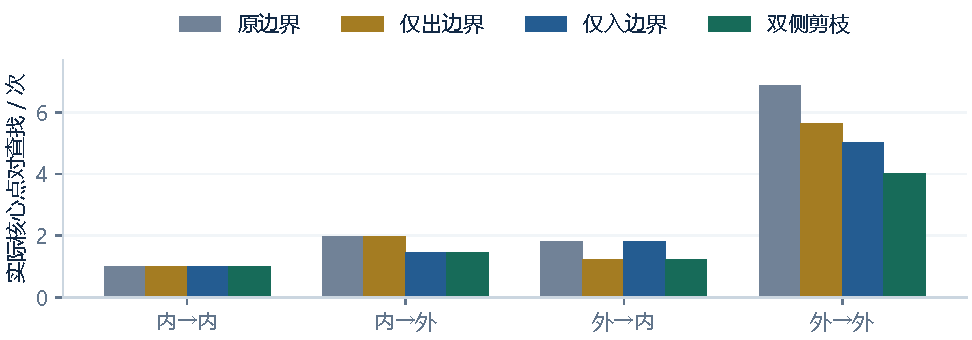
\includegraphics[width=.97\textwidth,height=44mm,keepaspectratio]{case_probes.pdf}\par
{\fontsize{11}{13}\selectfont 双侧剪枝将平均核心查找由 2.01 次降至 1.43 次，减少 29\%。\par 两端均在覆盖内时，查找过程保持不变。}
\end{frame}

\begin{frame}{查询性能与额外开销}
\framesubtitle{$k=4$，在相同混合编码下比较剪枝前后}
\centering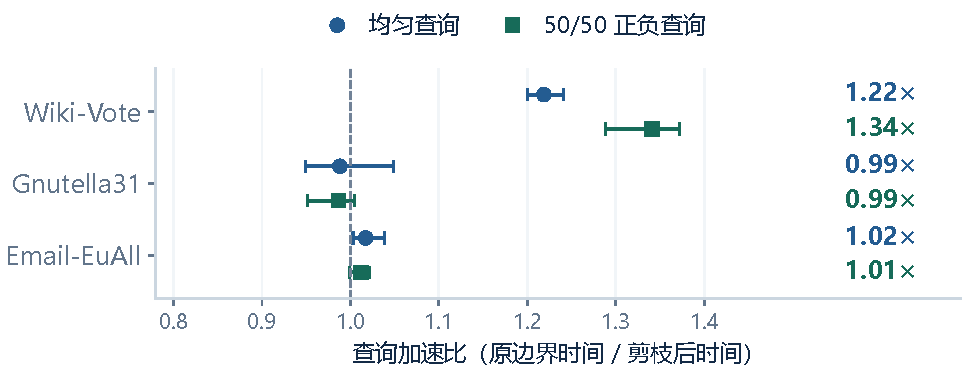
\includegraphics[width=.97\textwidth,height=44mm,keepaspectratio]{pruning_speed.pdf}\par
{\fontsize{11}{13}\selectfont Wiki 上平均加速 1.28 倍；P2P 和 Email 的查询时间变化较小。\par Wiki 增加约 70 KiB 边界索引，构建约 0.10s。}
\end{frame}

\section{总结}
\begin{frame}{总结与创新点}
\begin{columns}[T,onlytextwidth]
\column{.47\textwidth}
\begin{block}{论文的主要贡献}
用顶点覆盖连接任意查询端点，以三档距离信息支持四类精确查询，在索引规模和查询效率之间取得平衡。
\end{block}
\column{.47\textwidth}
\begin{block}{我们的改进}
按有限跳数下的集合支配约简查询边界，为两个预算、两个方向分别保存代表，并通过见证替代保持精确判定。
\end{block}
\end{columns}
\par\vspace{3mm}
实验表明，该方法在冗余边界较多的 Wiki 上减少了核心查找，并获得约 \WikiPruningSpeed{} 倍查询加速。\par\vspace{2mm}
后续可以优化边界构建的暂存空间，并结合构建开销选择适合启用剪枝的节点。
\par\vspace{2mm}\hfill 谢谢
\end{frame}


\appendix
\section{问答附录}

\begin{frame}{附录 A · 四类查询的正确性}
\fontsize{11}{14}\selectfont
\textbf{充分性：}核心距离不超过 $k-a-b$，接回起点与终点的 $a,b\in\{0,1\}$ 跳边，就得到长度不超过 $k$ 的行走；去环后仍有合法路径。\par\vspace{2mm}
\textbf{必要性：}合法路径的覆盖外起点首步必进入 $S$，覆盖外终点末步必来自 $S$。因此路径必经四类查询枚举的一对核心点，其最短核心距离满足剩余预算。\par\vspace{2mm}
\textbf{边界处理：}先处理 $s=t$；核心对角线保留零距离。两个外部端点共享一个核心邻居时也能正确接受。$k=1$ 可直接查边，本项目索引实验使用 $k\ge2$。
\Key{任意合法路径均对应一个满足预算的核心点对。}
\end{frame}

\begin{frame}{附录 B · 固定 $k$ 的索引与多 $k$ 查询}
假设在 $k=6$ 时建索引：\par\vspace{2mm}
$d(u,v)=2$ 与 $d(u,v)=4$ 都编码成 \T{01}，即“$d\le4$”。\par\vspace{2mm}
改问 $k=3$ 时，两者答案不同，原码却无法区分。\par\vspace{3mm}
原文 §4.4 讨论多 $k$ 的扩展；保存完整核心距离与三档码是不同设计。本项目 $k=2,4,6$ 分别编码，也分别构造预算相关边界。
\Key{固定 $k$ 下仍须区分两个预算：\T{Case 2/3 用 $k-1$，Case 4 用 $k-2$}。}
\end{frame}

\begin{frame}{附录 C · 原文 $(h,k)$-Reach 的空间—时间取舍}
\fontsize{11}{14}\selectfont
\textbf{$h$-hop 顶点覆盖：}每条长度为 $h$ 的路径至少含一个覆盖点。核心可以更小，但外部端点可能要走 $1\ldots h$ 跳接入核心。\par\vspace{2mm}
核心预算相应变为 $k-i-j$，需要保留更多距离阈值；原文定义给出 $h<k/2$。\par\vspace{2mm}
Nasa 的 $h=2,\mu=7$ 满足条件：覆盖 $1841\to1223$，百万查询从 $18.23\to39.48$ms。$\mu$ 为图上最短路径长度中位数。
\Key{更小的覆盖减少索引规模，同时增加端点接入核心的搜索开销。}
\end{frame}

\begin{frame}{附录 D · 核心编码是对照因素，单独控制}
\fontsize{11}{14}\selectfont
原文 §4.3 已讨论压缩。我们实现两位类别打包 CSR 与按行稀疏/稠密的 Hybrid，用作物理表示对照；\textbf{主图比较相同 Hybrid 上剪枝前后}。\par\vspace{2mm}
稀疏行载荷约 $4r+\lceil r/4\rceil$ 字节，稠密行 $\lceil |S|/4\rceil$ 字节。计入元数据后，混合布局不如两种全局格式时整体回退。\par\vspace{2mm}
原边界在所有新对照中均预先转为核心 ID，使用相同答案核。CSR 求交另有原边界和剪枝边界两个版本。
\Key{分别比较相同编码和相同查询方式下的剪枝效果。}
\end{frame}

\begin{frame}{附录 E · 部署空间、证书暂存与预处理分摊}
{\fontsize{9}{11}\selectfont\centering\begin{tabular*}{\textwidth}{@{\extracolsep{\fill}}lrrrrr@{}}\toprule
图 & 原边界/MiB & 剪枝/MiB & 总部署/MiB & 构建/s & 证书/MiB\\\midrule
Wiki-Vote & 0.10 & 0.17 & 2.01 & 0.10 & 2.52\\
Gnutella31 & 0.71 & 1.42 & 22.99 & 2.23 & 155.47\\
Email-EuAll & 3.37 & 6.63 & 34.74 & 5.04 & 314.92\\
\bottomrule\end{tabular*}\par}\par\vspace{2mm}
\fontsize{10.5}{13}\selectfont
总部署包含核心索引、节点映射和边界。证书用于离线构建，完成后可释放。Email 的核心距离暂存矩阵约为 1.23 GiB。\par\vspace{2mm}
原边界两个预算复用数组；剪枝后的预算列表分别保存，因此可能增加空间。
\Key{面向静态图上的重复查询，\T{预处理与额外存储是明确代价}。}
\Micro{Wiki $k=4$：按构建时间 0.10s 与当前平均查询节省估算，约 1.92 百万次查询可分摊构建开销。}
\end{frame}

\begin{frame}{附录 F · 不同 $k$ 下，结构相关收益也会变化}
\centering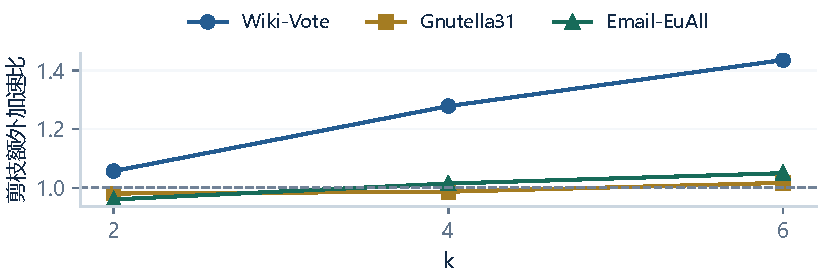
\includegraphics[width=.98\textwidth,height=44mm,keepaspectratio]{k_pruning.pdf}\par
\Key{每个 $k$ 分别建立两层预算边界；收益受阈值包含关系与原始查询工作共同影响。}
\end{frame}

\begin{frame}{附录 G · 更换覆盖构造，结论是否只依赖一次选择？}
\centering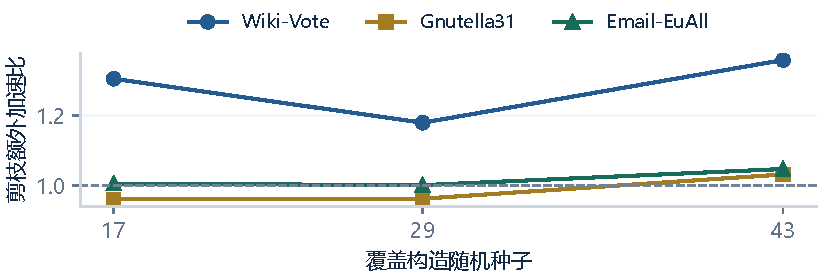
\includegraphics[width=.98\textwidth,height=44mm,keepaspectratio]{cover_pruning.pdf}\par
\Key{覆盖种子 17 / 29 / 43 全部保留，未按测试计时挑选覆盖；Wiki 在三次覆盖下均有收益。}
\end{frame}

\begin{frame}{附录 H · 单侧与双侧剪枝的时间消融}
\centering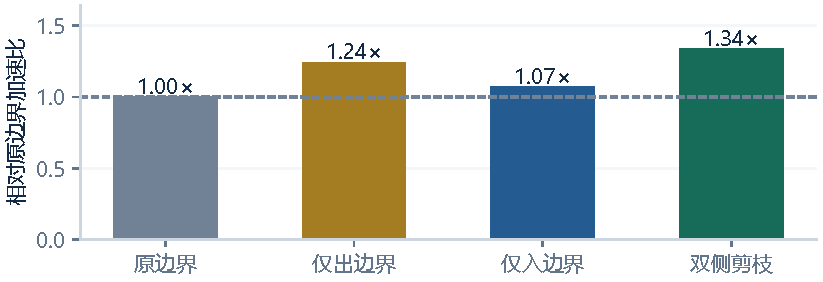
\includegraphics[width=.98\textwidth,height=44mm,keepaspectratio]{ablation.pdf}\par
\Key{出、入边界贡献不同；双侧同时保留阈值见证，再由实际计时判断整体收益。}
\end{frame}

\begin{frame}{附录 I · 所有图与 $k$ 的完整查询结果}
{\fontsize{8.5}{11}\selectfont\centering\begin{tabular*}{\textwidth}{@{\extracolsep{\fill}}llrrrrrr@{}}\toprule
图 & $k$ & Join & +剪枝 & 加速 & Hybrid & +剪枝 & 加速\\\midrule
Wiki-Vote & 2 & 0.550 & 0.557 & 0.99 & 0.425 & 0.403 & 1.06\\
Wiki-Vote & 4 & 0.429 & 0.379 & 1.13 & 0.246 & 0.191 & 1.28\\
Wiki-Vote & 6 & 0.363 & 0.302 & 1.20 & 0.212 & 0.145 & 1.43\\
Gnutella31 & 2 & 0.263 & 0.262 & 1.00 & 0.281 & 0.287 & 0.98\\
Gnutella31 & 4 & 0.344 & 0.349 & 0.98 & 0.357 & 0.361 & 0.99\\
Gnutella31 & 6 & 0.516 & 0.516 & 1.00 & 0.272 & 0.267 & 1.02\\
Email-EuAll & 2 & 0.416 & 0.423 & 0.98 & 0.420 & 0.437 & 0.96\\
Email-EuAll & 4 & 0.366 & 0.379 & 0.97 & 0.251 & 0.247 & 1.01\\
Email-EuAll & 6 & 0.339 & 0.333 & 1.02 & 0.232 & 0.221 & 1.05\\
\bottomrule\end{tabular*}\par}
\Micro{时间单位：$\mu$s/查询。Join / Hybrid 各自配对比较，避免把换编码的收益算到剪枝上。}
\end{frame}

\begin{frame}{附录 J · 后续研究与本项目分别优化什么？}
\fontsize{11}{14}\selectfont
\textbf{VCRea / VCRea$^+$（Tang 等，2023）}\par
以顶点覆盖构造两跳距离标签，给高出度点扩展 out-label、高入度点扩展 in-label，将标签对比较次数限制在至多 $d^2$。增加标签是一种空间与枚举代价取舍。\par\vspace{3mm}
\textbf{阈值支配剪枝（本项目）}\par
不增加距离精度，按现有两档阈值集合的包含关系消去冗余邻居；代价是边界构建及额外列表。\par\vspace{2mm}
近期 CSUR 综述单列 hop-constrained 语义，说明普通可达索引不能直接替代跳数约束。
\Key{VCRea 扩展距离标签；本项目研究固定 K-Reach 索引上的边界约简。}
\end{frame}

\begin{frame}{附录 K · 双侧约简的正确性}
\fontsize{11}{14}\selectfont
原出/入边界为 $A,B$，保留代表为 $A',B'$。任意合法核心对 $(y,v)$，满足 $d(y,v)\le b$。\par\vspace{2mm}
\textbf{替代源侧：}有 $x\in A'$，使 $R_b(y)\subseteq R_b(x)$。因此 $v\in R_b(x)$，即 $d(x,v)\le b$。\par\vspace{2mm}
\textbf{替代终侧：}有 $v'\in B'$，使 $L_b(v)\subseteq L_b(v')$。既然 $x\in L_b(v)$，就有 $d(x,v')\le b$。\par\vspace{2mm}
保留边界又是原边界的子集，所以不存在新增的错误成功见证。单侧分支只做相应的一次替代。
\Key{两侧必须用\T{相同剩余预算}，且终侧用前驱集合；普通可达或任意 SCC 代表不满足此条件。}
\end{frame}

\begin{frame}{附录 L · 构建方法与查找次数的变化}
\fontsize{10.5}{13}\selectfont
按集合大小降序处理邻居；已被保留集合包含就消去。反射性给出必要条件：\par
\[
R_b(y)\subseteq R_b(x)\ \Rightarrow\ d(x,y)\le b .
\]
先做该常数检查，再验证位集合包含。真实图审计使用\textbf{直接整数距离}逐项核对被消去者与其保留代表，独立于位打包构建。\par\vspace{2mm}
潜在候选上界不会增加，但找到成功见证的顺序可能变化。主实验及覆盖补充中，有 5 条查询的实际查找次数增加。
\Key{代表点可能出现在更后的位置，因此部分查询会在更多次检查后找到成功见证。}
\end{frame}

\begin{frame}{附录 M · 受控合成图上的机制验证}
\centering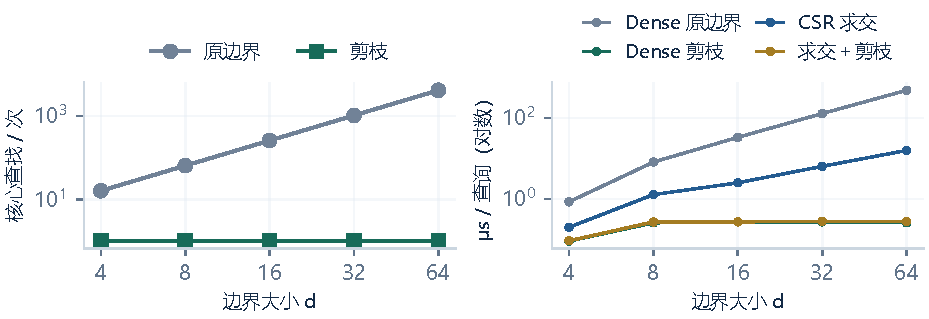
\includegraphics[width=.98\textwidth,height=50mm,keepaspectratio]{synthetic.pdf}\par
\Key{嵌套边界负例：原查找 $d^2$ 次，约简后 1 次。\T{固定全稠密 lookup 也有候选增长问题。}}
\end{frame}

\begin{frame}{参考文献}
\fontsize{9.5}{12}\selectfont
\begin{enumerate}\setlength\itemsep{3mm}
\item J. Cheng, Z. Shang, H. Cheng, H. Wang, J. X. Yu. \textbf{K-Reach: Who is in Your Small World.} \emph{PVLDB} 5(11):1292–1303, 2012. \href{https://doi.org/10.14778/2350229.2350247}{doi:10.14778/2350229.2350247}.
\item X. Tang, J. Zhou, Y. Shi, X. Liu, K. Lin. \textbf{Efficient Processing of k-Hop Reachability Queries on Directed Graphs.} \emph{Applied Sciences} 13(6):3470, 2023. \href{https://doi.org/10.3390/app13063470}{doi:10.3390/app13063470}.
\item C. Zhang, A. Bonifati, M. T. \"Ozsu. \textbf{Indexing Techniques for Graph Reachability Queries.} \emph{ACM CSUR} 58(6), Article 156, 2026; online Dec. 2025. \href{https://doi.org/10.1145/3776737}{doi:10.1145/3776737}.
\item J. Leskovec, A. Krevl. \textbf{SNAP Datasets}. \href{https://snap.stanford.edu/data/}{snap.stanford.edu/data/}.
\end{enumerate}
\end{frame}



\end{document}
